%%%% NeurReps 2026 — Proceedings Track (archival, double-blind) %%%%
\documentclass[mlmain,onecolumn]{jmlr}

% Watermark — remove for camera-ready
\usepackage[hpos=300px,vpos=70px]{draftwatermark}
\SetWatermarkText{}
\SetWatermarkScale{1}
\SetWatermarkAngle{0}

% amsmath, amssymb, natbib, graphicx, url, algorithm2e are auto-loaded
\usepackage{booktabs}

\def\R{\mathbb{R}}
\newcommand{\Ham}{H}
\newcommand{\flip}{R}

\jmlrvolume{}
\jmlryear{2026}
\jmlrworkshop{Symmetry and Geometry in Neural Representations}

\title[Time-Reversal Symmetry for Flow-Map Surrogates]{Symplectic Is Not Enough:
Time-Reversal Symmetry Makes Learned Flow Maps Usable as Hamiltonian Monte Carlo Proposals}

% Authors omitted for double-blind review.

\begin{document}

\maketitle

\begin{abstract}
Surrogate Hamiltonian Monte Carlo replaces an expensive log-density gradient
with a learned approximation. Every such method we are aware of learns a
\emph{vector field} --- a gradient, or an energy that is differentiated --- and
places it inside a symplectic integrator. This inherits the integrator's
correctness for free, but it also inherits its cost: advancing $L$ leapfrog
steps requires $L$ sequential network evaluations. A learned \emph{flow map}
needs one, independently of $L$. We show why this substitution is not free, and
what is required to make it sound. A Hamiltonian flow carries two structures:
it preserves the symplectic form, and it is time-reversal symmetric. Symplectic
networks encode the first by architecture and the second not at all --- and it
is the second that a Metropolis correction consumes, in the form of an
involution. An unsymmetrized symplectic network therefore violates detailed
balance by $\mathcal{O}(10^{-1})$, and no amount of training data repairs it.
Composing the network with its momentum-conjugate inverse restores the missing
symmetry exactly, as an algebraic identity in the weights and at no cost in
parameters; the construction is that of \citet{valperga2022reversible}, which we
transfer from dynamics prediction to the sampling setting and instantiate with
closed-form inverses for the LA- and G-SympNet layers. We further show that the
usual all-pairs training set is not merely unnecessary but harmful: supervising
only the single time offset the sampler queries is $1275\times$ cheaper at
$L=50$ and fits better. On Gaussian-process hyperparameter inference at the
benchmark configuration of \citet{Li_2019}, the resulting sampler attains
$3.7\times$ the effective samples per second of exact HMC, while every
integrator-based surrogate we test is \emph{slower} than exact HMC. We also
report a cautionary result: an unsymmetrized network posts a competitive
$142$ ESS/s at a reversibility error of $5\times10^{-4}$, illustrating that
effective sample size alone cannot certify a surrogate sampler.
\end{abstract}

\begin{keywords}
symplectic neural networks, Hamiltonian Monte Carlo, time-reversal symmetry,
structure-preserving architectures, surrogate models
\end{keywords}

\section{Introduction}

Structure-preserving architectures encode a known property of a physical system
into a hypothesis class, so that it holds for every choice of weights rather
than being approached through training. Symplectic neural networks
\citep[SympNets;][]{jin2020sympnets} are a clean instance: each layer is a shear
on phase space, so the network is symplectic by construction and its Jacobian
has unit determinant identically. They sit in a broader effort to learn
Hamiltonian dynamics with architectural constraints
\citep{greydanus2019hamiltonian,chen2019neural}.

Hamiltonian dynamics, however, carry more than one structure. Writing
$z = (q,p)$ and $\flip(q,p) = (q,-p)$ for the momentum flip, the exact flow
$\Phi_t$ of a Hamiltonian even in the momentum satisfies both
\begin{equation}
    \Phi_t^{*}\,(dq \wedge dp) = dq \wedge dp
    \qquad\text{and}\qquad
    \flip \circ \Phi_t \circ \flip = \Phi_t^{-1}.
    \label{eq:two-structures}
\end{equation}
The first is symplecticity; the second is time-reversal symmetry. A SympNet
inherits the first from its architecture. It does not inherit the second, and
the usual training objective --- a regression of predicted onto observed states
--- does not reward it.

We study the setting where this omission is not a matter of accuracy but of
correctness, and where it also has a concrete payoff: surrogate Hamiltonian
Monte Carlo.

\paragraph{Why one would want a learned flow map.}
Hamiltonian Monte Carlo \citep{Brooks_2011} proposes states by integrating
Hamiltonian dynamics and corrects the discretization error with a Metropolis
step. When the target's gradient is expensive, surrogate methods learn a cheap
stand-in during warm-up: a gradient \citep{Li_2019}, or a Hamiltonian that is
differentiated \citep{DHULIPALA2023112425}. In every such method the learned
object is a \emph{vector field} placed inside a symplectic integrator. That
inheritance is why they remain asymptotically exact --- an inaccurate network
lowers the acceptance rate but cannot bias the chain --- but it also fixes their
cost: advancing $L$ leapfrog steps costs $L$ sequential network evaluations.

A learned flow map is different in exactly this respect. Because
$\hat\phi(z,\tau)$ takes the elapsed time as an input, a proposal costs one
evaluation regardless of $L$. The saving grows with trajectory length, which is
precisely the regime adaptive schemes such as NUTS \citep{hoffman2011nouturn}
and ChEES \citep{hoffman2021adaptive} push towards. The obstacle is that
replacing the integrator forfeits the correctness it was supplying, and the
network must now provide that structure itself.

\paragraph{Contributions.}
\begin{itemize}
    \item We show that a SympNet used as an MCMC proposal satisfies volume
    preservation but violates involutivity, by $\mathcal{O}(10^{-1})$ at
    initialization and up to $\mathcal{O}(10^{0})$ after training
    (Table~\ref{tab:validity}). The resulting sampler is not asymptotically
    exact, and additional data does not fix it.
    \item We transfer the reversible-symplectic construction of
    \citet{valperga2022reversible} from dynamics prediction to sampling, and
    instantiate it with closed-form inverses for the LA- and G-SympNet layers,
    making it exact rather than approximate. We restate why it satisfies both
    Metropolis conditions (Proposition~\ref{prop:involution}) and is consistent
    (Lemma~\ref{lem:consistency}).
    \item We show that the standard all-pairs training set for flow maps is
    actively harmful: supervising only the offset the sampler queries is
    $1275\times$ cheaper at $L=50$ and yields \emph{higher} effective sample
    size (Table~\ref{tab:pairs}).
    \item Empirically, the symmetrized flow map attains $3.7\times$ the ESS/s
    of exact HMC on GP hyperparameter inference, where every integrator-based
    surrogate is slower than exact HMC (Figure~\ref{fig:results}a), with the
    advantage growing in $L$ (Figure~\ref{fig:results}b).
\end{itemize}

\section{Background}

\subsection{Validity of a deterministic Metropolis proposal}

Let $\pi(z) \propto e^{-\Ham(z)}$ on $\R^{2D}$ with $\Ham \circ \flip = \Ham$.
A Metropolis--Hastings scheme proposing $z' = T(z)$ deterministically and
accepting with probability $\min\{1, e^{\Ham(z) - \Ham(Tz)}\}$ leaves $\pi$
invariant provided
\begin{align}
    \text{(V)} \quad & |\det \nabla T(z)| = 1, \label{eq:vol}\\
    \text{(I)} \quad & (\flip \circ T) \circ (\flip \circ T) = \mathrm{Id},
    \label{eq:inv}
\end{align}
volume preservation and involutivity of $\flip \circ T$
\citep{Green1995,Tierney1998}. Leapfrog integration of any position-dependent
force satisfies both identically. That neural MCMC proposals must be engineered
to satisfy them is established \citep{song2017nice,levy2018generalizing}, and
\citet{spanbauer2020involutive} give a general construction from
volume-preserving involutions. Our observation is that the SympNet family,
adopted precisely for its structural guarantees, supplies \eqref{eq:vol} and
not \eqref{eq:inv}.

\subsection{Symplectic networks}

A SympNet composes layers that update either $q$ or $p$ using a function of the
other, unmodified half of the state; for the gradient module in ``up'' mode,
$(q,p) \mapsto (q,\; p + \tau\, K^{\!\top} a\, \sigma(Kq + b))$. Each layer has
unit-determinant Jacobian, so \eqref{eq:vol} holds for any weights.
Condition~\eqref{eq:inv} concerns how the map interacts with $\flip$, and no
layer constrains it.

\section{Symmetrizing the flow map}

\subsection{Closed-form inverses}

The shear structure that makes SympNets symplectic also makes them exactly
invertible. In an ``up'' layer the position passes through untouched, so the
increment added to $p$ can be recomputed from the output and subtracted; the
inverse is the same expression with the sign reversed, at identical cost and
with no iteration. The LA module applies a shear followed by a translation, so
its inverse subtracts the translation first and then undoes the shears in
reverse order. Composing layer inverses in reverse order gives $\Phi_t^{-1}$
exactly; we measure $\|\Phi_t^{-1}\Phi_t z - z\|_\infty \approx 10^{-15}$ in
double precision. \citet{valperga2022reversible} build their reversible
architecture from H\'enon maps and coupling layers; the SympNet modules admit
the same treatment, which lets the construction be applied to networks already
in use for Hamiltonian learning.

\subsection{The symmetrized map}

Following \citet{valperga2022reversible}, define
\begin{equation}
    \Psi_t \;:=\; \flip \circ \Phi_{t/2}^{-1} \circ \flip \circ \Phi_{t/2}.
    \label{eq:psi}
\end{equation}

\begin{proposition}
\label{prop:involution}
If $\Phi_{t/2}$ is invertible then $\Psi_t$ satisfies \eqref{eq:inv}; if it is
additionally symplectic then $\Psi_t$ satisfies \eqref{eq:vol}. The
Metropolis--Hastings chain with proposal $\Psi_t$ therefore leaves $\pi$
invariant for arbitrary network weights.
\end{proposition}

\begin{proof}
Write $\Phi := \Phi_{t/2}$. Since $\flip^2 = \mathrm{Id}$,
$\flip \circ \Psi_t = \Phi^{-1} \circ \flip \circ \Phi$, a conjugation of the
involution $\flip$, hence an involution:
$(\flip \Psi_t)^2 = \Phi^{-1}\flip\,\Phi\,\Phi^{-1}\flip\,\Phi
= \Phi^{-1}\flip^2\Phi = \mathrm{Id}$, which is \eqref{eq:inv}. For
\eqref{eq:vol}, $\flip$ is anti-symplectic, so $\flip \Phi^{-1} \flip$ is
symplectic and $\Psi_t$, a composition of two symplectic maps, is symplectic;
hence $|\det \nabla \Psi_t| = 1$. Neither argument uses any property of $\Phi$
beyond invertibility and symplecticity.
\end{proof}

\begin{lemma}
\label{lem:consistency}
If $\Phi_s$ is the exact time-$s$ flow of a Hamiltonian with
$\Ham \circ \flip = \Ham$, then $\Psi_t = \Phi_t$.
\end{lemma}

\begin{proof}
By \eqref{eq:two-structures}, $\Phi_{t/2}^{-1} = \flip \Phi_{t/2} \flip$;
substituting into \eqref{eq:psi} and using $\flip^2 = \mathrm{Id}$ gives
$\Psi_t = \Phi_{t/2}\circ\Phi_{t/2} = \Phi_t$.
\end{proof}

Equation~\eqref{eq:psi} is the adjoint (symmetrization) composition of geometric
integration \citep{HairerLubichWanner}, with the adjoint realized as
$\flip \circ \Phi^{-1} \circ \flip$. The property survives composition: if
$\flip \Psi \flip = \Psi^{-1}$ then $\flip \Psi^{k} \flip = \Psi^{-k}$, so
$(\flip \Psi^{k})^2 = \mathrm{Id}$ for every $k$, and multi-step trajectories
remain valid proposals. The map costs two network evaluations rather than one
and adds no parameters; note that a $\Psi$ built from an $n$-block network has
the same effective depth as a plain $2n$-block network, so comparisons must
control for effective depth rather than block count.

\subsection{What the sampler actually queries}

Flow maps are conventionally trained on all pairs $(x_i, x_j)$, $i<j$, drawn
from each warm-up trajectory, giving $\mathcal{O}(L^2)$ examples per trajectory.
But the sampler evaluates $\hat\phi$ at exactly one offset, $\tau = L\epsilon$.
The extra offsets are not free: with finite capacity, fitting times the sampler
never queries takes capacity from the one it does. Table~\ref{tab:pairs}
compares supervising all pairs, all offsets from $x_0$, and only $(x_0, x_L)$.

\begin{table}[t]
\centering
\caption{Pair construction for the symmetrized flow map (Gaussian target).
Supervising only the queried offset is dramatically cheaper \emph{and} fits
better as $L$ grows.}
\label{tab:pairs}
\begin{tabular}{llrrrr}
\toprule
$L$ & pairs & per traj. & total & train (s) & ESS \\
\midrule
5  & all        & 15   & 9\,000   & 10.0 & 762 \\
5  & from $x_0$ & 5    & 3\,000   & 7.8  & 763 \\
5  & endpoint   & 1    & 600      & 7.7  & 709 \\
\midrule
25 & all        & 325  & 195\,000 & 72.0 & 352 \\
25 & from $x_0$ & 25   & 15\,000  & 23.3 & 348 \\
25 & endpoint   & 1    & 600      & 20.1 & \textbf{1175} \\
\midrule
50 & all        & 1275 & 765\,000 & 72.4 & 429 \\
50 & from $x_0$ & 50   & 30\,000  & 37.3 & 267 \\
50 & endpoint   & 1    & 600      & 36.3 & \textbf{711} \\
\bottomrule
\end{tabular}
\end{table}

\section{Experiments}

Models are trained on warm-up trajectories from exact HMC and used as proposals,
corrected with the exact Hamiltonian. All models share an optimization protocol
(Adam at $10^{-2}$, learning rate halved on plateau, early stopping,
best-iterate restoration), so comparisons reflect architecture rather than
tuning. Timings are measured on an isolated GPU.

\paragraph{Structural validity.}
Table~\ref{tab:validity} evaluates \eqref{eq:vol} and \eqref{eq:inv} directly at
random initialization, emphasizing that these are properties of the construction
and not of training. Integrator-based surrogates satisfy both to machine
precision. Plain SympNets satisfy volume preservation and violate involutivity
by $\mathcal{O}(10^{-1})$. The symmetrized versions satisfy both.

\begin{table}[t]
\centering
\caption{Validity conditions at random initialization ($D=2$, $L=5$,
$\epsilon=0.1$, double precision). Volume preservation is
$\max|{\det \nabla T}|-1$; involutivity is $\max\|(\flip T)^2 z - z\|_\infty$.}
\label{tab:validity}
\begin{tabular}{lccc}
\toprule
proposal map & $|\det \nabla T| - 1$ & involution error & valid \\
\midrule
Exact leapfrog (HMC)                  & $2\cdot10^{-16}$ & $3\cdot10^{-16}$ & yes \\
Learned force $+$ leapfrog            & $3\cdot10^{-16}$ & $7\cdot10^{-16}$ & yes \\
Learned separable $\Ham$ $+$ leapfrog & $7\cdot10^{-16}$ & $1\cdot10^{-15}$ & yes \\
Learned field $+$ leapfrog            & $8\cdot10^{-16}$ & $9\cdot10^{-16}$ & yes \\
\midrule
LA-SympNet (plain)                    & $1\cdot10^{-15}$ & $2.4\cdot10^{-1}$ & \textbf{no} \\
G-SympNet (plain)                     & $7\cdot10^{-16}$ & $1.2\cdot10^{-1}$ & \textbf{no} \\
LA-SympNet (symmetrized)              & $2\cdot10^{-15}$ & $4\cdot10^{-16}$ & yes \\
G-SympNet (symmetrized)               & $7\cdot10^{-16}$ & $1\cdot10^{-16}$ & yes \\
\bottomrule
\end{tabular}
\end{table}

\begin{figure}[t]
\centering
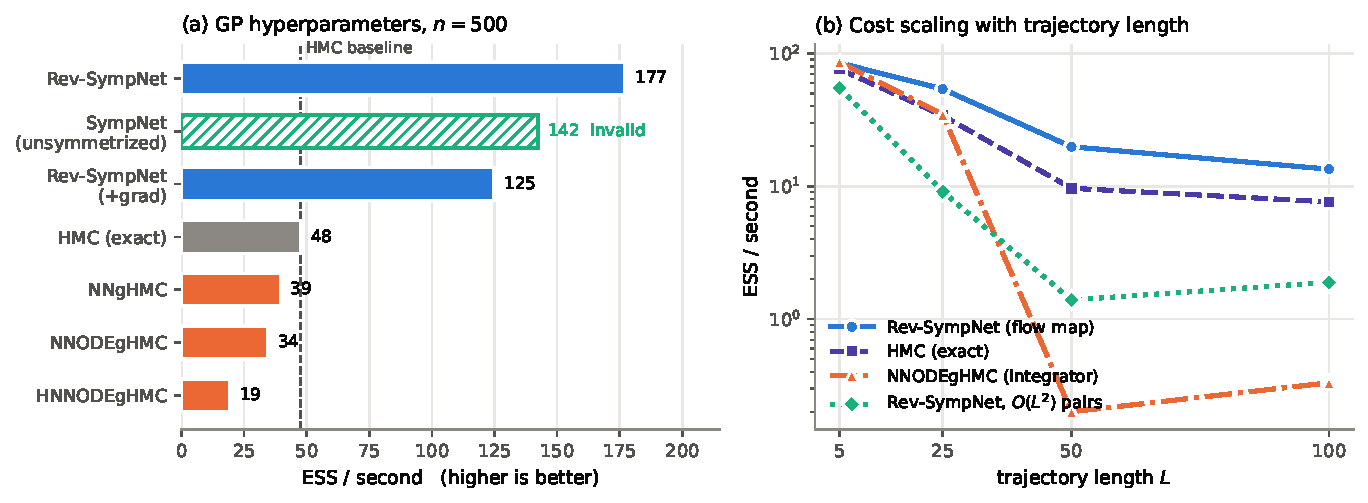
\includegraphics[width=\textwidth]{results.pdf}
\caption{(a) Gaussian-process hyperparameter inference at the configuration of
\citet{Li_2019} ($n=500$, Mat\'ern $\nu=3/2$, $\epsilon=0.05$, $L=20$, $10^4$
samples); best value over training budgets. The symmetrized flow map attains
$3.7\times$ the ESS/s of exact HMC, while every integrator-based surrogate is
slower than exact HMC. The unsymmetrized network (hatched) posts a competitive
number at a reversibility error of $5\times10^{-4}$ and is not a valid sampler.
(b) ESS/s against trajectory length. The flow map's advantage grows with $L$;
the integrator-based surrogate collapses because it compounds error over $L$
steps; and training on $\mathcal{O}(L^2)$ pairs erases the gain.}
\label{fig:results}
\end{figure}

\paragraph{Expensive-likelihood target.}
We use GP hyperparameter inference at the configuration of \citet{Li_2019}:
$n=500$ observations with four features, a Mat\'ern kernel with $\nu = 3/2$, two
sampled hyperparameters, $\epsilon = 0.05$, $L=20$, $10^4$ samples. Each
gradient requires an $\mathcal{O}(n^3)$ Cholesky factorization.
Figure~\ref{fig:results}a reports the best ESS/s over training budgets. The
symmetrized flow map reaches $177$ ESS/s against exact HMC's $48$, a factor of
$3.7$; the gain is wall-clock, not sample quality, since HMC attains higher raw
ESS ($18\,634$ versus $11\,609$) in $6\times$ the time. Every integrator-based
surrogate is slower than exact HMC ($0.41$--$0.83\times$).

\paragraph{Scaling with trajectory length.}
Figure~\ref{fig:results}b varies $L$ on a Gaussian target. The symmetrized flow
map exceeds exact HMC at every $L$, by $2.05\times$ at $L=50$. The
integrator-based surrogate degrades sharply --- its ESS falls to $20.5$ at
$L=50$ --- because it applies its learned field $L$ times and compounds error at
each step, whereas the flow map applies once. Training on all pairs removes the
advantage entirely, consistent with Table~\ref{tab:pairs}.

\paragraph{Effective sample size does not certify a surrogate.}
In Figure~\ref{fig:results}a the unsymmetrized network attains $142$ ESS/s,
which would read as a $3\times$ improvement over exact HMC, at a reversibility
error of $5\times 10^{-4}$. A map with a large involution defect can produce
weakly autocorrelated paths while targeting the wrong distribution; ESS measures
autocorrelation, not correctness. Structural diagnostics of the kind in
Table~\ref{tab:validity} should accompany any reported ESS for a learned
proposal. We note this because the artifact is easy to mistake for a result.

\section{Discussion}

The observation we wish to emphasize is structural. When an architecture is
called structure-preserving it is worth asking which structures, and whether the
intended use requires others. SympNets preserve the symplectic form exactly and
are adopted for that reason, but the flows they model are also time-reversal
symmetric, and it is that second symmetry an accept--reject correction consumes.
Because it can be imposed exactly by composition, at no cost in parameters and
with no loss of consistency, there is little reason to leave it to training.

Two limitations bound our claims. First, our targets are low-dimensional (two to
thirty parameters); the flow map must represent a map on the full
$2D$-dimensional phase space, whereas gradient-learning surrogates fit a field
on the $D$-dimensional position space alone, and we would expect that gap to
widen with dimension. Second, our speedups are measured on GPU, where a
$500\times500$ Cholesky costs about $4$\,ms and the gradient is not the dominant
per-step cost; \citet{Li_2019} report a $39.3\times$ speedup for a
gradient-learning surrogate on their hardware, which we do not reproduce
($0.83\times$) at matched $n$ and $L$. Our advantage comes from a different
mechanism --- collapsing $L$ sequential operations into one --- and the two
numbers are not comparable.

Finally, supervising only the queried offset makes the map fast and accurate but
fixes the trajectory length at training time. Adaptive-length schemes
\citep{hoffman2011nouturn,hoffman2021adaptive} would require the $\mathcal{O}(L)$
construction, at a measurable cost in fit; making trajectory length adaptive for
a flow map --- where, unlike for an integrator, length carries no per-proposal
cost --- is the natural next question.

\bibliography{neurreps}

\end{document}
